\section{Introduction}\label{sec:introduction}

Reasoning models such as DeepSeek-R1~\cite{deepseekr1} and QwQ~\cite{qwq} can ``self-jailbreak'': their chain of thought transitions from safety-aware deliberation to committed harmful generation without adversarial input~\cite{harmthoughts,selfjailbreak}. We call the first reasoning step after which safety deliberation permanently ceases the \textbf{Safety Commitment Point} (CP). Existing safety detectors operate at the token or input level~\cite{trajguard,safeswitch,saferemind}, missing the gradual, multi-step commitment process within reasoning traces. Hidden-state (HS) probing offers a natural alternative for step-level monitoring, but requires choosing which transformer layer to read. This choice is typically treated as an implementation detail.\looseness=-1

We show it determines whether the probe appears to succeed or fail (\cref{fig:concept_overview}). Across four models, two architectures, and two scales (\cref{tab:models}), a crossing-rate composite metric systematically selects shallow layers (L0--L10), where HS and text probes perform equivalently. Threshold-based metrics select deep layers (L14--L63), where HS probes gain +20--22pp precision, cross-validated at 7--8B. The divergence spans 14 to 61 layers. The mechanism is cosine compression (\cref{fig:cosine_compression}): shallow layers compress step-to-step directional information by 1.4--2.7$\times$, inflating frequency-based metrics near the noise floor. This bias generalizes across all models, a second dataset (AdvBench), and a fifth architecture (Gemma-2).\looseness=-1

\begin{figure*}[t]
\centering
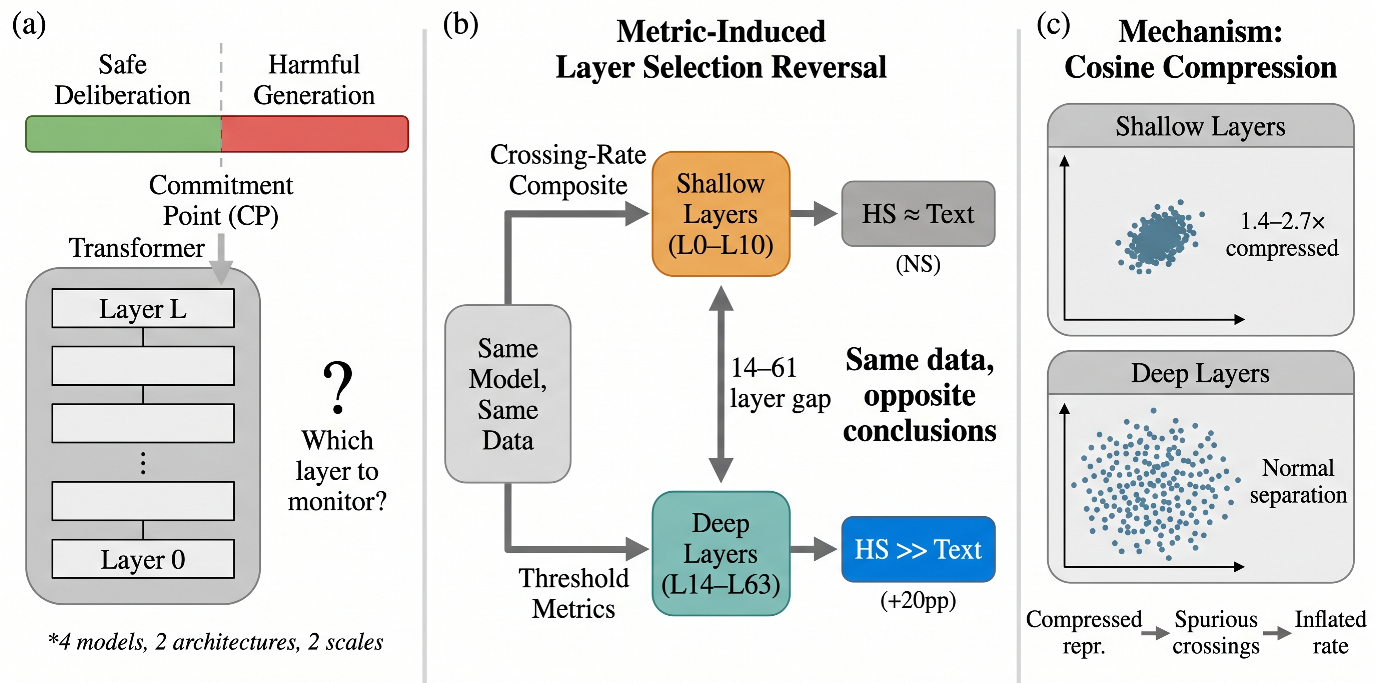
\includegraphics[width=0.95\textwidth]{figures/fig_concept_overview.pdf}
\caption{Metric-induced layer selection reversal. The same hidden states, evaluated with different layer selection metrics, yield opposite conclusions about the hidden-state advantage. Crossing-rate composite selects shallow layers (L0--L10), where hidden-state and text probes perform equivalently; threshold-based metrics select deep layers (L14--L63), where hidden-state probes significantly outperform text (+20pp). The 14--61 layer gap arises from the metric alone.}
\label{fig:concept_overview}
\end{figure*}

The HS advantage at correctly selected layers is conditional: it narrows from 4/4 to 1/4 significant models with stronger text encoders (384d vs.\ 1024d) and remains suggestive at 32B due to small samples ($n \leq 20$). Seven alternative detection methods, including Bayesian online change-point detection (BOCPD), representation engineering (RepE), contrastive consistency search (CCS), and cross-model transfer, all fail to match supervised probing. Control tasks confirm the probes exploit genuine safety structure rather than superficial statistical patterns.\looseness=-1

Our contributions are threefold. \textbf{(C1)~Metric-induced layer selection bias}: crossing-rate composite metrics systematically select shallow layers, producing a qualitative reversal of the hidden-state advantage; we trace the mechanism to cosine compression and show it generalizes across models and datasets (AdvBench); the geometric precondition extends to a fifth architecture (Gemma-2). \textbf{(C2)~Boundary conditions on the hidden-state advantage}: cross-validated at 7--8B, conditional on encoder quality, and suggestive at 32B. \textbf{(C3)~Comprehensive negative results}: seven alternative methods all fail, establishing supervised temporal probing with principled layer selection as the current best approach.\looseness=-1
